\documentclass[11pt,a4paper]{article}

% -------------------------------------------------------------------------

\usepackage{kotex}
\usepackage{amsmath}
\usepackage{amssymb}
\usepackage{array}
\usepackage{booktabs}
\usepackage{longtable}

\usepackage[hidelinks,colorlinks=true,linkcolor=magenta,citecolor=magenta,urlcolor=blue]{hyperref}

\usepackage{graphicx}
\usepackage{caption}
\usepackage{subcaption}
\setlength{\textfloatsep}{25pt plus 2pt minus 4pt}
\setlength{\floatsep}{25pt plus 2pt minus 2pt}
\setlength{\intextsep}{25pt plus 2pt minus 2pt}

\usepackage{geometry}
\geometry{margin=25mm}

\usepackage{titlesec}
\titlespacing*{\section}{0pt}{5ex plus 1ex minus .2ex}{2ex}
\titlespacing*{\subsection}{0pt}{4ex plus 1ex minus .2ex}{1ex}
\titlespacing*{\subsubsection}{0pt}{3ex plus .8ex minus .2ex}{1ex}
\setcounter{secnumdepth}{3}
\titleformat{\section}{\large\bfseries}{\thesection}{0.5em}{}
\titleformat{\subsection}{\normalsize\bfseries}{\thesubsection}{0.5em}{}
\titleformat{\subsubsection}{\normalsize\bfseries}{\thesubsubsection}{0.5em}{}

\usepackage{setspace}
\setstretch{1.2}

\usepackage{indentfirst}

% -------------------------------------------------------------------------

\makeatletter
\newcommand{\subtitle}[1]{\gdef\@subtitle{#1}}
\newcommand{\studentinfo}[1]{\gdef\@studentinfo{#1}}
\def\@subtitle{}
\def\@studentinfo{}
\renewcommand{\maketitle}{%
  \begin{center}
    {\LARGE\bfseries \@title\par}
    \vspace{0.5em}
    {\large \@subtitle\par}
  \end{center}
  \vspace{-1.0em}
  \begin{flushright}
    \normalsize \@studentinfo
  \end{flushright}
}
\makeatother

% -------------------------------------------------------------------------

\begin{document}

\title{Open Source Lab 2 - In-Memory Database}
\subtitle{Open Source SW Analysis (BigData) 2분반}
\studentinfo{
소속 학과: 소프트웨어학과\\
학번: 32220222\\
이름: 구현모\\
제출일: 2026-04-06
}

\maketitle

\section{과제 개요}
본 과제의 목표는 RocksDB의 in-memory 구조를 단순화한 형태로 구현하면서 skip list 기반 memtable의 동작을 이해하고, 추가로 B+Tree 기반 구조를 직접 구현하는 것이다. 필수 과제에서는 skip list를 memtable로 사용하며 out-of-place update, sequence number, tombstone, mutable/immutable memtable 관리가 핵심이다. 보너스 과제에서는 하나의 큰 B+Tree를 사용하고, delete가 실제 노드 삭제로 이어지는 in-place update 구조를 구현해야 한다. 구현 방향을 정리할 때 RocksDB Wiki의 memtable 설명과 skip list 자료, 그리고 B+Tree 고전 문헌을 참고했다.

구현은 \texttt{repo/lab2/skiplist}와 \texttt{repo/lab2/bptree}를 기준으로 진행했다. 최종 제출용 소스는 과제 요구사항에 맞춰 \texttt{memdb.cc}, \texttt{memdb.h}, \texttt{skiplist.cc}, \texttt{skiplist.h}, 그리고 보너스용 \texttt{bptree.cc}, \texttt{bptree.h}만 별도 tar로 정리했다.

\section{구현 내용}
\subsection{Skip list 기반 In-Memory DB}
\subsubsection{Skip list 구조}
\texttt{skiplist.cc}에서는 각 노드가 \texttt{key}, \texttt{seq}, \texttt{value}, \texttt{tombstone}, \texttt{next}, \texttt{down}을 가지도록 설계했다. 최상위부터 최하위까지 sentinel head를 미리 생성하고, 삽입 시 동전 던지기 방식의 \texttt{RandomLevel()}로 타워 높이를 정한다. 동일 key에 대해서는 최신 버전이 먼저 발견되어야 하므로 \texttt{key}가 같을 때 \texttt{seq}가 큰 노드가 앞에 오도록 정렬 기준을 정의했다.

\subsubsection{Put, Get, Delete}
\texttt{Put()}은 삽입 경로를 \texttt{update} 벡터에 저장한 뒤, 생성된 높이만큼 새 노드를 연결한다. 이때 \texttt{next\_seq\_}를 증가시키며 버전 순서를 보존한다. \texttt{Get()}은 최하위 레벨에서 특정 key의 첫 번째 노드를 찾고, 해당 노드가 tombstone이면 삭제된 key로 간주하여 실패를 반환한다. \texttt{Delete()}는 실제 노드를 제거하지 않고 tombstone 노드를 새 버전으로 삽입한다. RocksDB의 memtable처럼 최신 삭제가 오래된 값을 가려야 하므로 이 방식이 필요하다.

\subsubsection{Range scan}
\texttt{RangeScan()}은 내부적으로 \texttt{RangeEntries()}를 사용한다. 최하위 레벨에서는 같은 key의 여러 버전이 연속으로 배치되므로, 범위 탐색 중 같은 key를 처음 만난 항목만 채택하면 최신 버전을 얻을 수 있다. 그 결과 skip list 내부 range scan에서는 tombstone을 제외한 유효 key-value만 반환한다.

\subsubsection{Memtable 관리}
\texttt{memdb.cc}에서는 mutable memtable 하나와 immutable memtable들의 벡터를 관리한다. \texttt{Put()}과 \texttt{Delete()} 전에 \texttt{EnsureMutableCapacity()}를 호출해 현재 memtable이 \texttt{max\_memtable\_bytes}를 넘길 경우 immutable로 전환하고 새 mutable memtable을 만든다.

\texttt{Get()}은 mutable부터 시작해서 최신 immutable 순으로 탐색한다. 특정 memtable에서 tombstone을 발견하면 그보다 오래된 memtable은 볼 필요가 없으므로 즉시 실패를 반환한다. \texttt{RangeScan()}은 모든 memtable을 최신 순으로 검사하면서 이미 본 key를 \texttt{seen} 집합에 기록하고, tombstone이 아닌 첫 항목만 결과 집합에 반영한다. 이를 통해 여러 memtable에 걸친 최신 값만 반환되도록 했다.

\subsection{B+Tree 기반 In-Memory DB}
\subsubsection{노드 구성}
\texttt{bptree.h}의 \texttt{Node}는 leaf 여부, key 배열, leaf 전용 value 배열, 자식 포인터 배열, leaf 간 연결을 위한 \texttt{next} 포인터를 가진다. 내부 노드는 자식 포인터만 보유하고, \texttt{keys[i]}는 \texttt{children[i+1]} 서브트리의 최소 key를 의미하도록 유지했다. 이 구조를 사용하면 자식 선택과 range scan이 단순해진다.

\subsubsection{삽입과 split}
\texttt{Put()}은 재귀 함수 \texttt{Insert()}를 호출한다. leaf에서는 정렬 위치를 찾아 key를 삽입하고, 이미 존재하는 key면 value만 덮어쓴다. leaf가 최대 key 수(\texttt{degree-1})를 초과하면 중간 지점에서 오른쪽 leaf를 분리하고 \texttt{next} 포인터를 갱신한다. 내부 노드에서는 분할된 오른쪽 자식을 부모의 \texttt{children}에 삽입한 뒤 separator key를 다시 계산한다. 자식 수가 최대 차수(\texttt{degree})를 넘으면 내부 노드도 같은 방식으로 분할한다.

\subsubsection{삭제와 rebalance}
\texttt{Delete()}는 leaf에서 key를 제거한 뒤, 최소 key 수 조건을 깨는 경우 부모에서 \texttt{RebalanceChild()}를 호출한다. 먼저 왼쪽 형제, 그 다음 오른쪽 형제에게서 빌릴 수 있는지 확인한다. 빌리기가 불가능하면 leaf끼리 merge하고, 내부 노드도 동일한 원리로 자식을 병합한다. 병합이나 차용 후에는 \texttt{RefreshInternalKeys()}로 부모 separator key를 즉시 다시 계산한다. 루트가 내부 노드이면서 자식이 하나만 남으면 높이를 한 단계 줄이고, 루트 leaf가 비면 전체 트리를 비운다.

\subsubsection{탐색과 range scan}
\texttt{Get()}은 \texttt{FindLeaf()}로 대상 leaf를 찾은 뒤 이진 탐색으로 value를 조회한다. \texttt{RangeScan()}은 시작 key가 포함될 leaf를 찾고, 이후에는 leaf linked list를 따라 순차적으로 이동하면서 범위 끝 key까지 결과를 수집한다. B+Tree의 모든 데이터가 leaf에 저장되므로 이 방식이 가장 자연스럽다.

\section{실험 및 고찰}
\subsection{실험 목적}
skip list 기반 memtable에서 \texttt{max\_memtable\_bytes} 크기가 읽기 성능에 어떤 영향을 주는지 확인했다. memtable이 작으면 immutable memtable 수가 늘어나고, \texttt{Get()}이 더 많은 skip list를 순차 탐색해야 하므로 읽기 지연이 커질 것으로 예상했다.

\subsection{실험 환경}
\begin{table}[h]
\centering
\begin{tabular}{ll}
\toprule
항목 & 값 \\
\midrule
OS & macOS Darwin 25.3.0 arm64 \\
Compiler & Apple clang 17.0.0 \\
대상 프로그램 & \texttt{repo/lab2/skiplist/memdb\_bench} \\
Workload & \texttt{fillrandom}, \texttt{readrandom} \\
\texttt{num} & 100000 \\
\texttt{key\_range} & 100000 \\
\texttt{value\_size} & 100 byte \\
\texttt{skiplist\_p} & 0.5 \\
\texttt{skiplist\_height} & 16 \\
\bottomrule
\end{tabular}
\caption{실험 환경}
\end{table}

\subsection{실험 결과}
\begin{table}[h]
\centering
\begin{tabular}{rrrr}
\toprule
\texttt{memtable\_bytes} & FillRandom (sec) & ReadRandom (sec) & Read hit \\
\midrule
1,048,576  & 0.277623 & 4.083930 & 63,314 / 100,000 \\
4,194,304  & 0.378311 & 2.443740 & 63,314 / 100,000 \\
16,777,216 & 0.478226 & 1.446960 & 63,314 / 100,000 \\
\bottomrule
\end{tabular}
\caption{Memtable 크기에 따른 skip list 성능 변화}
\end{table}

\begin{figure}[h]
\centering
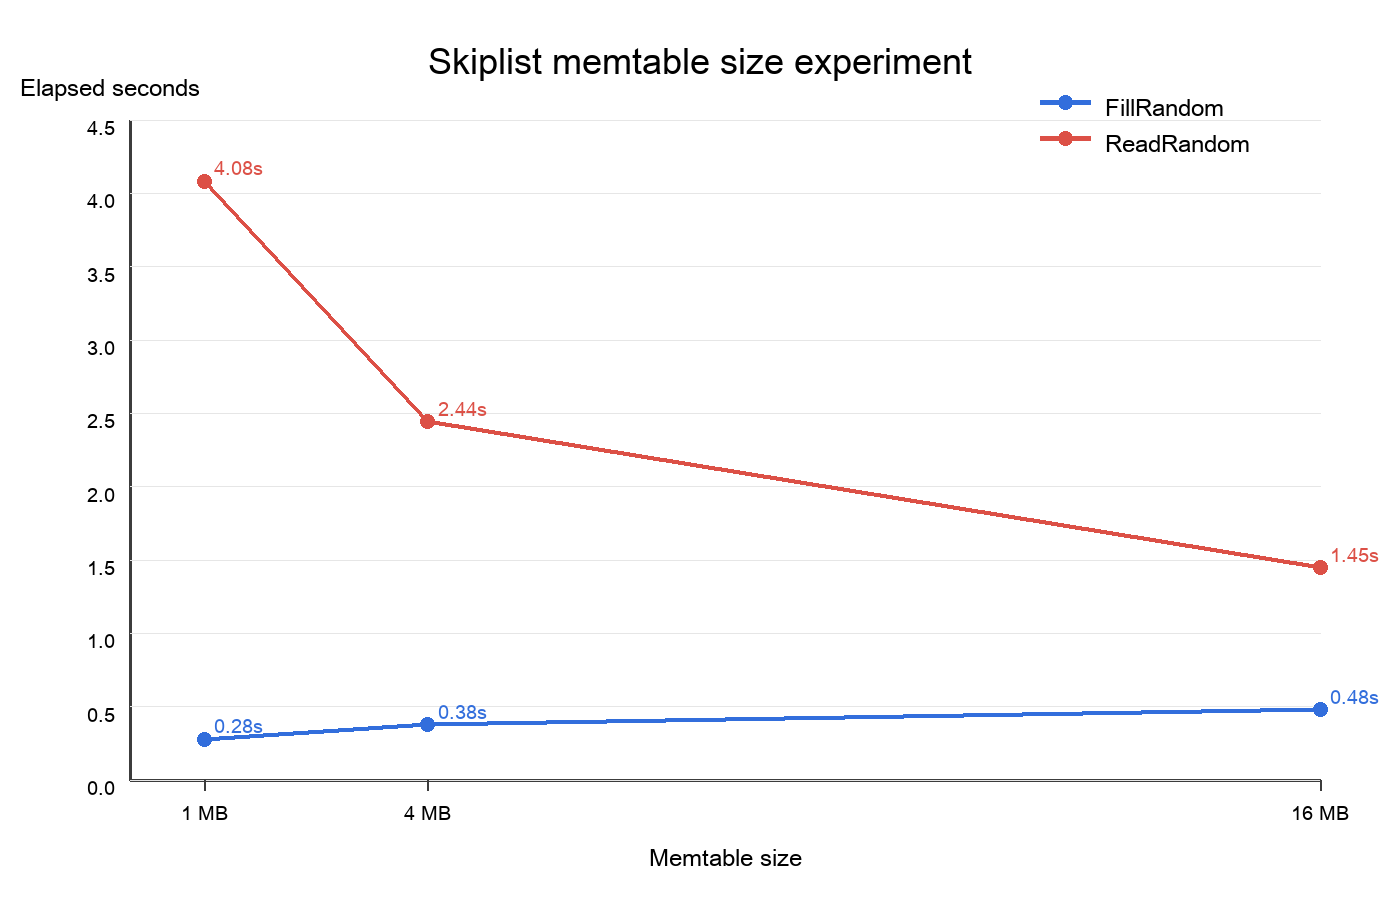
\includegraphics[width=0.88\linewidth]{lab2_skiplist_memtable_experiment.png}
\caption{Memtable 크기에 따른 FillRandom / ReadRandom 실행 시간}
\end{figure}

\subsection{결과 분석}
실험 결과 \texttt{memtable\_bytes}가 커질수록 \texttt{ReadRandom} 실행 시간이 뚜렷하게 감소했다. 1MB에서는 약 4.08초였고, 4MB에서는 약 2.44초, 16MB에서는 약 1.45초까지 줄었다. 이는 memtable 크기가 커질수록 immutable memtable로의 전환 횟수가 줄고, \texttt{Get()}이 확인해야 하는 memtable 수가 감소하기 때문이다.

반면 \texttt{FillRandom}은 memtable이 커질수록 다소 증가했다. 본 구현에서는 삽입 자체는 한 개의 mutable memtable에만 수행되지만, 큰 memtable일수록 하나의 skip list에 더 많은 노드가 누적되면서 평균 탐색 경로가 길어지고 캐시 지역성도 불리해질 수 있다. 따라서 쓰기 성능만 보면 작은 memtable이 약간 유리했지만, 읽기까지 고려하면 지나치게 작은 memtable은 전체 성능을 악화시킨다.

추가로 \texttt{read hit} 값이 세 실험에서 동일하게 나타난 점도 확인했다. workload와 난수 seed를 고정했기 때문에 저장된 key 집합 자체는 같고, memtable 크기는 데이터 배치 방식만 바꾸므로 hit ratio는 변하지 않는다. 즉 이번 실험에서 성능 차이는 데이터 정확성 문제가 아니라 memtable 수와 탐색 비용 차이에서 발생했다.

\subsection{구현 과정에서의 관찰}
skip list 과제의 핵심은 단순한 정렬 linked list 구현이 아니라, 버전 관리와 tombstone을 range scan까지 일관되게 반영하는 것이었다. \texttt{Get()}만 맞추고 \texttt{RangeScan()}에서 tombstone이나 오래된 값을 걸러내지 않으면 테스트는 일부만 통과하고 실제 동작은 RocksDB의 memtable과 달라진다. 따라서 skip list 내부의 최신 버전 판정과 memdb 레벨의 최신 memtable 우선 병합을 분리해 설계한 것이 중요했다.

보너스 B+Tree에서는 테스트 통과보다 구조 보존이 더 어려웠다. 특히 삭제 후 underflow를 처리할 때 형제 노드에서 빌릴 수 있는지, 아니면 merge해야 하는지에 따라 부모 separator key를 즉시 갱신해야 했다. 이를 위해 separator key를 직접 저장한 뒤 부분 수정하는 방식보다, 자식의 최소 key를 다시 읽어 \texttt{RefreshInternalKeys()}로 재계산하는 방식이 구현 실수를 줄였다.

\section{결론}
필수 과제에서는 skip list 기반 memtable과 sequence number, tombstone, mutable/immutable memtable 전환, 범위 검색까지 구현하여 RocksDB의 in-memory 동작을 단순화한 형태로 재현했다. 보너스 과제에서는 leaf linked list를 포함한 B+Tree를 구현하고 split, borrow, merge를 통해 균형을 유지하도록 만들었다.

실험에서는 memtable 크기가 읽기 성능에 직접적인 영향을 준다는 점을 확인했다. 작은 memtable은 flush 빈도를 높여 읽기 시 더 많은 immutable memtable을 탐색하게 만들었고, 큰 memtable은 읽기 성능을 개선했다. 반대로 쓰기 성능은 약간 손해를 볼 수 있으므로, 실제 시스템에서는 workload 성격에 맞는 memtable 크기 조정이 필요하다고 판단했다.

\begin{thebibliography}{9}
\bibitem{rocksdb-memtable}
Meta Platforms, Inc.,
\textit{RocksDB Wiki: MemTable},
\url{https://github.com/facebook/rocksdb/wiki/MemTable},
accessed 2026-04-06.

\bibitem{rocksdb-skiplist}
Meta Platforms, Inc.,
\textit{RocksDB Wiki: SkipList MemTable},
\url{https://github.com/facebook/rocksdb/wiki/Memtable#skiplist-memtable},
accessed 2026-04-06.

\bibitem{pugh-skiplist}
William Pugh,
\textit{Skip Lists: A Probabilistic Alternative to Balanced Trees},
Communications of the ACM, 33(6), 1990.

\bibitem{comer-btree}
Douglas Comer,
\textit{The Ubiquitous B-Tree},
ACM Computing Surveys, 11(2), 1979.
\end{thebibliography}

\end{document}
